\documentclass[a4paper]{article}
\usepackage[14pt]{extsizes} % для того чтобы задать нестандартный 14-ый размер шрифта
\usepackage[utf8]{inputenc}
\usepackage[english,main=russian]{babel}
\usepackage{setspace,amsmath}
\usepackage{subcaption}
\usepackage[final]{graphicx}
\usepackage{epstopdf}
\usepackage{mathtext}
\DeclareGraphicsExtensions{.pdf,.png,.jpg}
\usepackage[left=20mm, top=15mm, right=15mm, bottom=15mm, nohead, footskip=10mm]{geometry} % настройки полей документа
\usepackage{ragged2e}
\justifying

% =======================================================
% Далее титульный лист
% =======================================================

\begin{document}
\begin {center}
    \hfill \break
    \textbf{Федеральное государственное бюджетное образовательное учреждение высшего образования}\\
    \small{\textbf{«РЫБИНСКИЙ ГОСУДАРСТВЕННЫЙ АВИАЦИОННЫЙ ТЕХНИЧЕСКИЙ УНИВЕРСИТЕТ имени П. А. СОЛОВЬЁВА»}}\\
    \hfill \break
    \normalsize{Институт информационных технологий и систем управления}\\
    \hfill \break
    \normalsize{Кафедра математического и программного обеспечения электронных вычислительных средств}\\
    \hfill\break
    \hfill \break
    \hfill \break
    \hfill \break
    \large{Лабораторная работа №1}\\
    \normalsize{\textbf{"Знакомство с основами загрузки и обработки данных"}}\\
    \hfill \break
    \hfill \break
    \hfill \break
    \normalsize{по дисциплине\\
Методы и алгоритмы анализа данных\\}
    \hfill \break
    \hfill \break
    \hfill \break
    \hfill \break
    \hfill \break
\end {center}

\begin {flushleft}
\normalsize{ 
    Выполнили студенты 
    группы ИВМ-22  
    \hfill Перхуров В. А. \\
    \hfill Беляев А. Е. \\
    \hfill \break
    Проверил: 
    \hfill Кулиманов И. Е. 
}
\end {flushleft}

\hfill \break
\hfill \break
\hfill \break
\hfill \break
\hfill \break
\hfill \break
\hfill \break

\begin{center} 
    Рыбинск 2022 
\end{center}
\thispagestyle{empty} 

% =======================================================
% Далее лист с заданием
% =======================================================

\newpage
\begin{center}
    \hfill \break
    \textbf{Задание}\\
\end{center}  
\normalsize{
    \textbf{Постановка задачи:}\\\\
    Цели:\\\\
    Получить практические навыки по загрузке и обработке данных\\\\
    Задачи:\\
    \begin{enumerate}
        \item Загрузить датасет "MNIST".
        \item Вывести изображения нескольких случайных чисел.
        \item Загрузить датасет "Titanic".
        \item Выполнить ряд заданий по исследованию датасета:
        \begin{itemize}
            \item Проанализируйте датасет и создайте несколько диаграмм/гистограмм и объясните что они отображают.
            \item Заполните записи со значением NaN, объясните как заполняли.
            \item Создайте дополнительный признак, объясните для чего он необходим.
        \end{itemize}
    \end{enumerate}
}

% =======================================================
% Далее листы с описанием датасетов
% =======================================================

\newpage
\begin{center}
    \hfill \break
    \section{Описание датасетов}
\end{center}

\subsection{Описание датасета MNIST}
\normalsize{
    Файл данных содержит изображения нарисованных от руки цифр в оттенках серого от нуля до девяти.
    
    Каждое изображение имеет высоту 28 пикселей и ширину 28 пикселей, всего 784 пикселя. С каждым пикселем связано одно значение пикселя, указывающее яркость или темноту этого пикселя, причем более высокие числа означают темнее. Это значение пикселя представляет собой целое число от 0 до 255 включительно.
    
    Набор данных содержит 785 столбцов. Первый столбец, называемый «метка», представляет собой цифру, нарисованную пользователем. Остальные столбцы содержат значения пикселей связанного изображения.
    
    Каждый столбец пикселей в наборе имеет имя, например pixelx, где x — целое число от 0 до 783 включительно. Чтобы найти этот пиксель на изображении, предположим, что мы разложили x как
    \[x = i * 28 + j,\]
    где i и j — целые числа от 0 до 27 включительно.
    
    Затем pixelx находится в строке i и столбце j матрицы 28 x 28 (индексируется нулем).
    
    Например, pixel31 указывает пиксель, который находится в четвертом столбце слева и во второй строке сверху.
}

\subsection{Описание датасета Titanic}
\normalsize{
    Набор данных представлен в CSV-файле. Набор содержит признак Survived для каждого пассажира, обозначающий, выжил данный пассажир или нет (0 для умерших, 1 для выживших).
    
    Каждая строчка наборов данных содержит следующие поля:
    \begin{enumerate}
        \item Pclass — класс пассажира (1 — высший, 2 — средний, 3 — низший), 
        \item Name — имя, 
        \item Sex — пол, 
        \item Age — возраст, 
        \item SibSp — количество братьев, сестер, сводных братьев, сводных сестер, супругов на борту титаника,
        \item Parch — количество родителей, детей (в том числе приемных) на борту титаника,
        \item Ticket — номер билета,
        \item Fare — плата за проезд,
        \item Cabin — каюта,
        \item Embarked — порт посадки (C — Шербур; Q — Квинстаун; S — Саутгемптон).
    \end{enumerate}
     
    В поле Age приводится количество полных лет. Для детей меньше 1 года — дробное. Если возраст не известен точно, то указано примерное значение в формате xx.5.
}

% =======================================================
% Далее листы с описанием выполнения работы
% =======================================================

\newpage
\begin{center}
\hfill \break
\section{Описание выполнения работы}
\end{center}

\subsection{Реализация программы для анализа датасета MNIST}
\subsubsection{Используемые библиотеки}
\normalsize{
    При решении данной задачи были использованы следующие библиотеки:
    \begin{enumerate}
        \item random - генератор случайных чисел,
        \item pandas - анализ данных,
        \item numpy - математика и работа с массивами,
        \item PIL.Image - работа с изображениями.
    \end{enumerate}
}
\subsubsection{Ход работы и результат выполнения программы}
\normalsize{
    В ходе выполнения работы была написана консольная программа, которя выводит несколько (задаваемое число) случайных чисел из загруженного датасета.
    
    Пример работы данной программы показан на рисунке 1.
    \begin{figure}[h]
        \centering
        \graphicspath{{./}}
        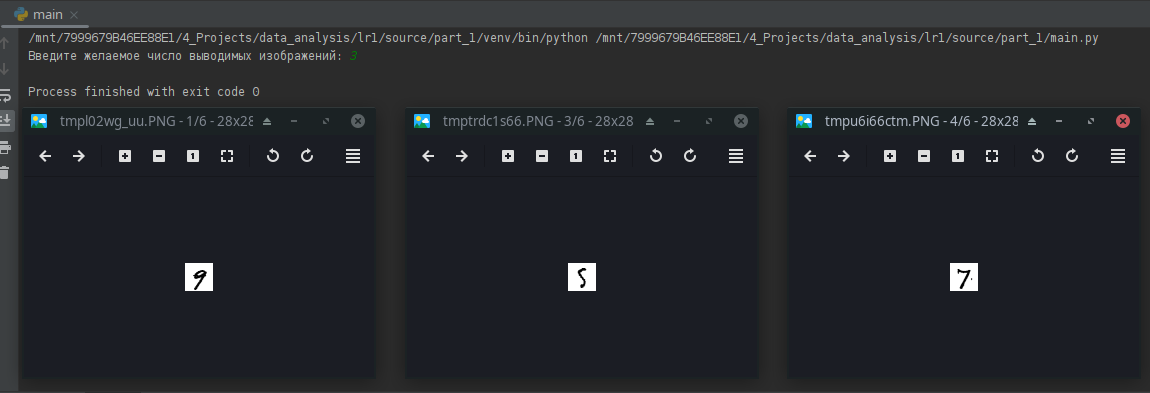
\includegraphics[scale=0.5]{run_program_1}
        \caption{Результат работы программы для вывода заданного числа изображений}
    \end{figure}
}
\subsubsection{Исходный текст программы}
\normalsize{
    \begin{verbatim}
import random  # генератор случайных чисел
import pandas as pd  # анализ данных
import numpy as np  # математика и работа с массивами
from PIL import Image  # работа с изображениями

# 1 - Вывести заданное количество случайных чисел
def showImage(df):
    result_mass = np.zeros((28, 28), dtype=np.uint8)
    index = random.randint(0, 4200)
    for i in range(0, 784, 1):
        result_mass[i//28, i%28] = 255 - df[f"pixel{i}"].values[index]
    Image.fromarray(result_mass).show()

def main():
    # 0 - Читаем датасет
    df = pd.read_csv('./numbers.csv', escapechar='`', low_memory=False)
    # 1 - Выводим заданное количество случайных чисел
    image_count = int(input("Введите желаемое число " 
                            "выводимых изображений: "))
    for i in range(0, image_count, 1):
        showImage(df)

main()
    \end{verbatim}
}

\subsection{Реализация программы для анализа датасета Titanic}
\subsubsection{Используемые библиотеки}
\normalsize{
    При решении данной задачи были использованы следующие библиотеки:
    \begin{enumerate}
        \item pandas - анализ данных,
        \item numpy - математика и работа с массивами,
        \item matplotlib.pyplot - построение графиков.
    \end{enumerate}
}
\subsubsection{Ход работы и результат выполнения программы}
\normalsize{
    В ходе выполнения работы была написана программа, которя выводит три гафика зависимостей (рисунок 2), построенных на основе данных из заданного датасета, и формирует дополнительный признак на основе имеющихся данных (рисунок 4).
    
    На рисунке 2 показаны три графика (слева направо):
    \begin{enumerate}
        \item Зависимость числа пассажиров взошедших на борт от порта посадки.
        \item Зависимость средней стоимости билетов и числа пассажиров от класса.
        \item Зависимость выручки от класса
    \end{enumerate}
    
    \begin{figure}[h]
        \centering
        \graphicspath{{./}}
        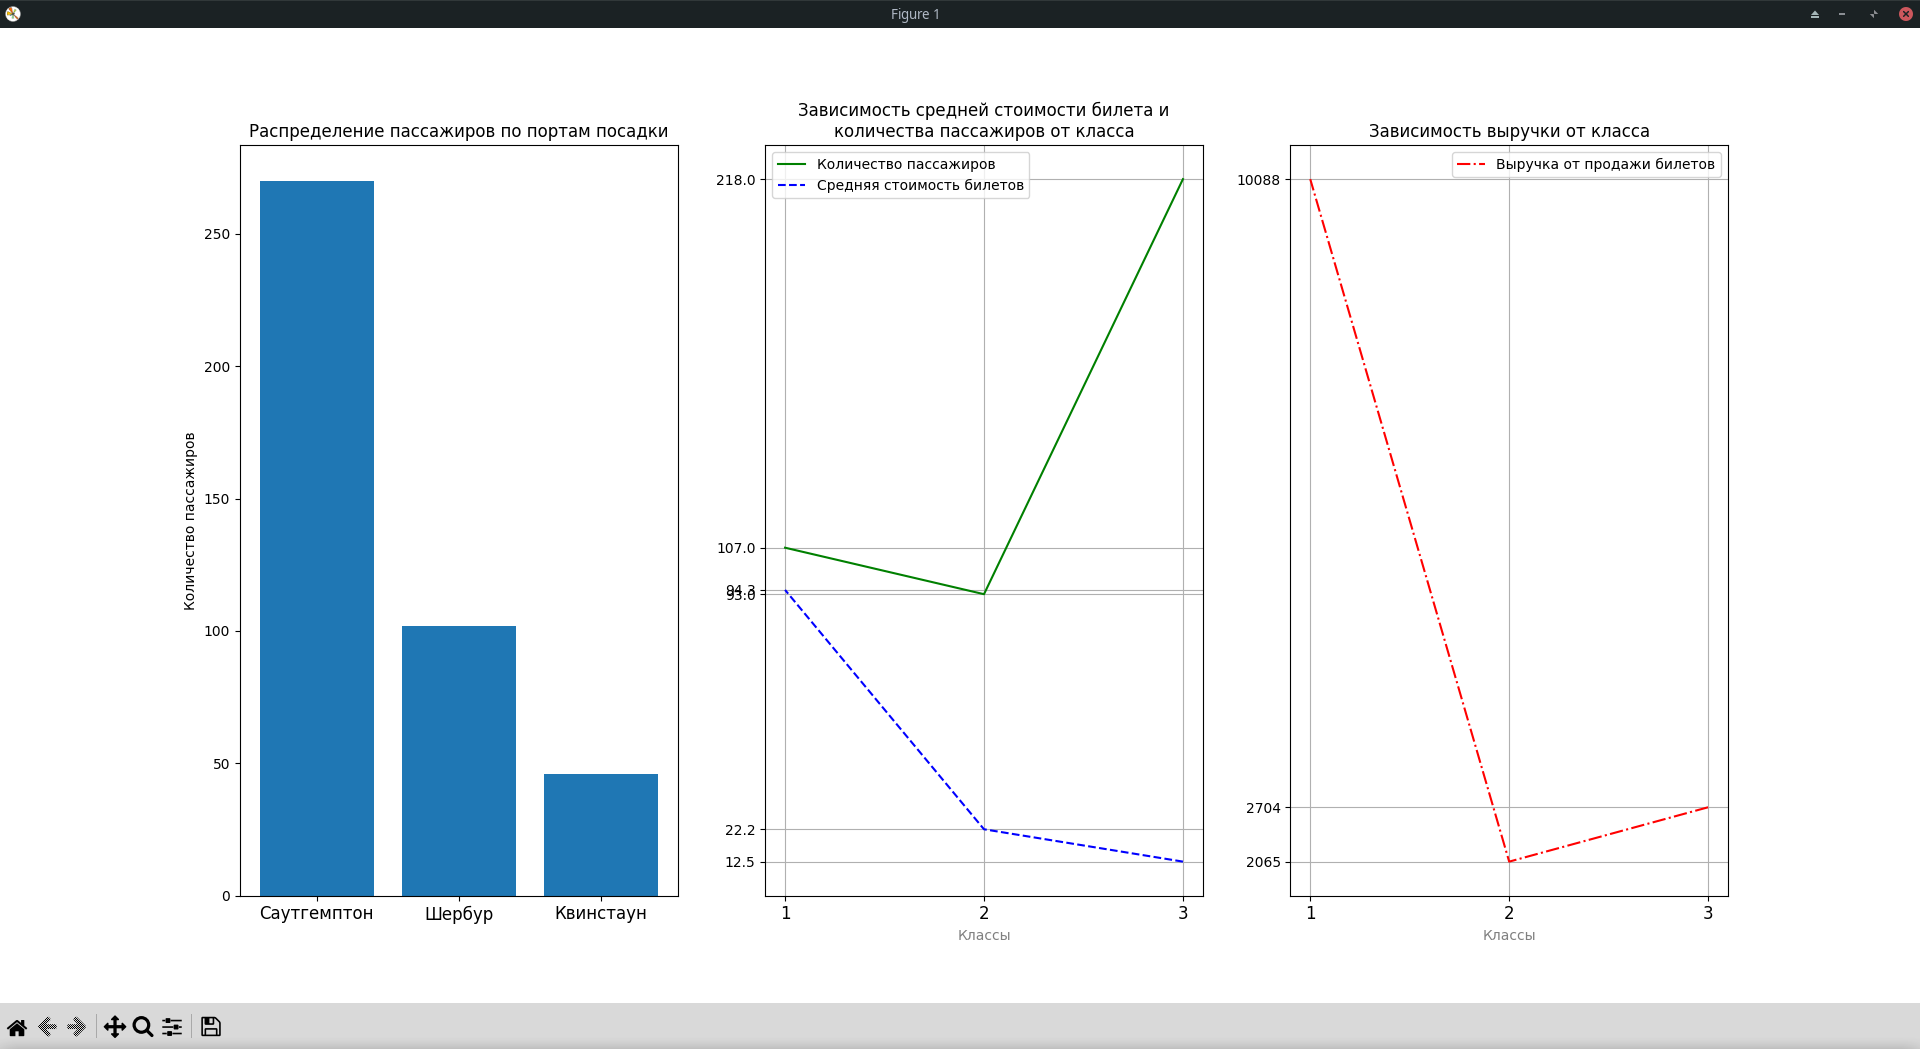
\includegraphics[scale=0.325]{run_program_2_diagram.png}
        \caption{Диаграммы, построенные при исполнении программы}
    \end{figure} 
    
    На рисунке 4 показан фрагмент изменённого датасета, где ячейки, содержащие значение NaN, были заполнены строкой "Unknown" с целью идентифкации факта неизвестности значения данного параметра для конкретной записи (пасажира). Замена производилось с помощью метода fillna.

    Так же был добавлен дополнительный признак - буквенный код палубы. Введение нового параметра - буквенного кода палубы, позволит в дальнейшем не производить анализ номера каюты для определения палубы, с целью использования её в дальнейшей обработке.
    
    \begin{figure}[h]
        \centering
        \graphicspath{{./}}
        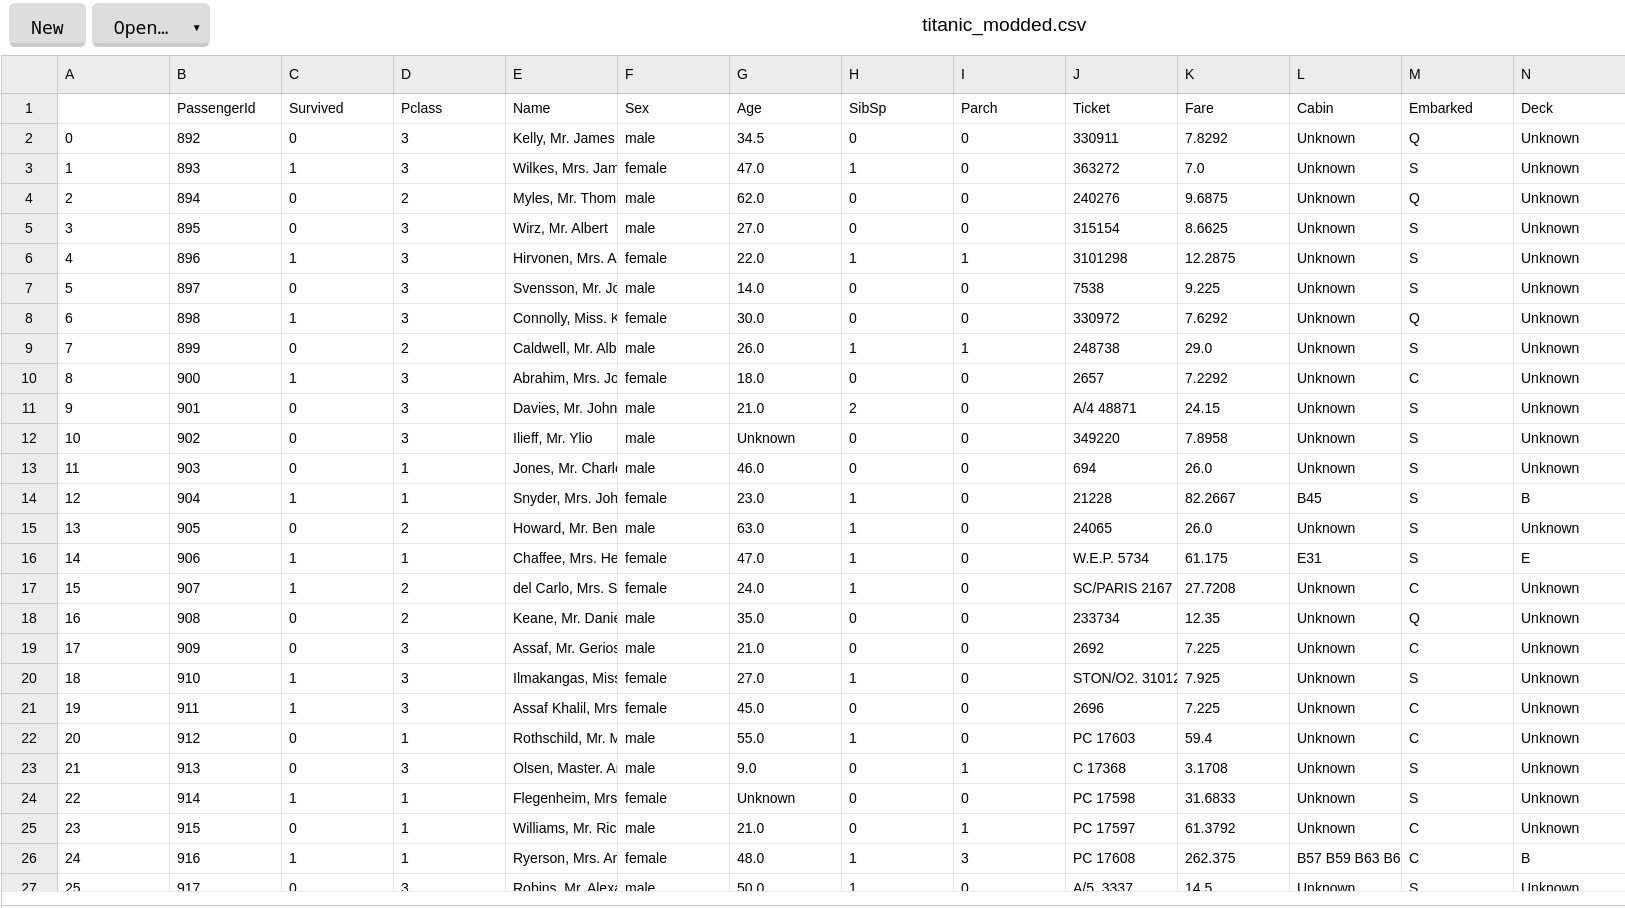
\includegraphics[scale=0.383]{run_program_2_modded_dataset.png}
        \caption{Результат внесения изменений в исходный датасет}
    \end{figure}
}
\subsubsection{Исходный текст программы}
\normalsize{
    \begin{verbatim}
import pandas as pd # анализ данных
import numpy as np # математика и работа с массивами
from matplotlib import pyplot as plt # построение графиков

# Получить списки ключей и значений из отсортированного 
# по убыванию словаря
def getKeysAndValues(dataset, with_sort):
    dict_dataset = dict(dataset)
    keys = []
    values = []
    if with_sort:
        dict_dataset = sorted(dict_dataset.items(),
                              key=lambda x: x[1],
                              reverse=True)
        for k, v in dict_dataset:
            keys.append(k)
            values.append(v)
    else:
        for k, v in dict_dataset.items():
            keys.append(k)
            values.append(v)
    return (keys, values)

# Отрисовать первую диаграмму.
# Зависимость числа пассажиров зашедших на борт от порта посадки.
# Зависимость средней стоимости билетов и числа пассажиров от класса.
# Зависимость выручки от класса.
def showDiagrams(main_df):
    # подсчёт числа пассажиров, взошедших на борт в городах
    boarding = pd.value_counts(main_df['Embarked'].values, sort=True)
    for i in range(0, len(boarding.index.values), 1):
        if boarding.index.values[i] == 'S':
            boarding.index.values[i] = 'Саутгемптон'
        else:
            if boarding.index.values[i] == 'C':
                boarding.index.values[i] = 'Шербур'
            else:
                boarding.index.values[i] = 'Квинстаун'

    boarding_keys, boarding_values = getKeysAndValues(boarding, True)
    top_boarding = len(boarding_keys)

    plt.subplot(131)
    plt.title('Распределение пассажиров по портам посадки')
    plt.bar(np.arange(top_boarding), boarding_values)
    plt.xticks(np.arange(top_boarding), 
               boarding_keys, 
               rotation=0,
               fontsize=12)
    plt.ylabel('Количество пассажиров')

    # подсчёт числа пассажиров по классам
    classes = pd.value_counts(main_df['Pclass'].values, sort=False)
    classes_keys, classes_values = getKeysAndValues(classes, False)

    # подсчёт средней стоимости билетов и общей выручки
    average_fare = {}
    revenue = {}
    for i in classes_keys:
        dfs = main_df[['Fare', 'Pclass']].loc[main_df['Pclass'] == i]
        average_fare[i] = dfs['Fare'].mean(axis=0)
        revenue[i] = dfs['Fare'].sum()
        
    average_fare_keys, average_fare_values =
        getKeysAndValues(average_fare, False)
    revenue_keys, revenue_values = getKeysAndValues(revenue, False)

    plt.subplot(132)
    plt.grid(True)
    plt.title('Зависимость средней стоимости билета и\n'
              'количества пассажиров от класса')
    plt.xticks(classes_keys, rotation=0, fontsize=12)
    plt.yticks(classes_values+average_fare_values)
    plt.xlabel('Классы', color='gray')
    plt.plot(classes_keys, classes_values, 'g',
             average_fare_keys, average_fare_values, 'b--')
    plt.legend(['Количество пассажиров','Средняя стоимость билетов'],
               loc=2)

    plt.subplot(133)
    plt.grid(True)
    plt.title('Зависимость выручки от класса')
    plt.xticks(classes_keys, rotation=0, fontsize=12)
    plt.yticks(revenue_values)
    plt.xlabel('Классы', color='gray')
    plt.plot(revenue_keys, revenue_values, 'r-.')
    plt.legend(['Выручка от продажи билетов'], loc=1)
    plt.show()

    return

# Заполнить поля значением Unknown.
# Ячейки, содержащие значение NaN, были заполнены строкой "Unknown" 
# с целью идентифкации факта неизвестности
# значения данного параметра для конкретной записи (пасажира). 
# Замена производилось с помощью метода fillna.
def fillNanFields(main_df):
    main_df = main_df.fillna('Unknown')
    return main_df

# Создать дополнительный признак (буквенного кода палубы).
# Введение нового параметра - буквенного кода палубы, позволит в
# дальнейшем не производить анализ номера каюты
# для определения палубы, с целью использования её в дальнейшей
# обработке.
def createAnAdditionalAttribute(main_df):
    main_df = main_df.assign(Deck=main_df.Cabin)
    for i in range(len(main_df.Deck)):
        if main_df.Deck[i] != 'Unknown':
            main_df.loc[i, 'Deck'] = main_df.loc[i, 'Deck'][:1]
            
    return main_df

# Основная функция
def main():
    # 0 - Читаем датасет
    df = pd.read_csv('./titanic.csv', escapechar='`', low_memory=False)
    # 1 - Рисуем диаграммы зависимостей
    showDiagrams(df)
    # 3 - Заполняем поля значением Unknown
    df = fillNanFields(df)
    # 4 - Создаём дополнительный признак
    df = createAnAdditionalAttribute(df)
    # 5 - Сохраняем изменнеия в новый файл
    df.to_csv('./titanic_modded.csv')

# Запускаем программу
main()
    \end{verbatim}
}
 
% =======================================================
% Далее лист с выводом о проделанной работе
% =======================================================

\newpage
\begin{center}
\hfill \break
\section{Вывод.}
\end{center} 
\normalsize{
    В результате выполнения лабораторной работы были получены навыки по загрузке и начальной обработке данных на примере двух датасетов.
    
    В ходе выполнения работы были написаны две программы (по одной на каждый датасет). Обе выполняют чтение датасетов из фалов в формате ".csv" и реализуют заданный функционал.
    
    Первая (для датасета "MNIST") формирует заданное число случайно выбранных изображений и выводит их на экран.
    
    Вторая (для датасета "Titanic") выполняет две операции:
    
    1. Анализ данных из датасета и вывод их в виде графиков.
    
    2. Изменение и добавление новых данных в имеющийся датасет и сохранение его в отдельный файл.
}
\end{document}